\section{Part B: Sample Means and Visualization}
\begin{itemize}

    \item Compute the sample means for each set of replicates. You should have 9 of them, 3 for each distribution with varying sample sizes.
    \item For each distribution and replicate size, we want to view and compare their distributions. Which plot do you think is appropriate? Plot the appropriate plot for each replicate, please plot them separately. 
    \item Do not confuse the distribution of sample mean with the distribution of the sample (which you plotted in Part A).
\end{itemize}
-----\\

For each set of replicates, I computed the sample mean across the 100 observations within each replicate. This resulted in 6 sets of sample means: 3 for the Uniform distribution (with 10, 100, and 1000 replicates) and 3 for the Pareto distribution (with 10, 100, and 1000 replicates). I'm guessing that having 9 of them is outdated, because 3 each from the 2 distributions is 6 sample means. The implementation is shown below:\\

\begin{verbatim}
def compute_sample_means(replicates_csv: str) -> np.ndarray:
    """
    Computes the sample mean for each replicate.
    
    :param replicates_csv: Path to CSV containing replicates
    :type replicates_csv: str
    :returns: Array of sample means, one per replicate
    :rtype: np.ndarray
    """
    df = pd.read_csv(replicates_csv)
    sample_means = df.mean(axis=0).to_numpy()
    return sample_means
\end{verbatim}

\begin{center}
\textbf{Figure 5:} Function for computing sample means from replicates.\\
\end{center}

To visualize the distribution of sample means, I chose to use histograms. This choice is best because histograms effectively visualize the shape and spread of the distribution mass of sample means, allowing us to best assess whether they appear to be approaching a normal distribution as the Central Limit Theorem predicts for larger numbers of replicate sample means. Since the whole point of this task is to gain insight about CLT, this plot ought to be the most appropriate to appreciate the convergence to Normal. The plotting function is shown below:

\begin{verbatim}
def plot_sample_means_distribution(sample_means: np.ndarray, dist_name: str, 
                                   replicate_size: int, output_filename: str):
    """
    Plots the distribution of sample means.
    
    :param sample_means: Array of sample means
    :type sample_means: np.ndarray
    :param dist_name: Name of the distribution
    :type dist_name: str
    :param replicate_size: Replicate size
    :type replicate_size: int
    :param output_filename: Output filename for figure
    :type output_filename: str
    """
    sns.set_style("whitegrid")
    sns.set_palette("muted")
    plt.figure(figsize=(10, 6))
    
    ax = sns.histplot(sample_means, bins=50, stat='density',
                     edgecolor='white', alpha=0.7)
    
    ax.set_xlabel('Sample Mean', fontsize=14, labelpad=15)
    ax.set_ylabel('Density', fontsize=14, labelpad=15)
    ax.set_title(f'Distribution of {dist_name} Sample Means of Replicate with size {replicate_size}',
                fontsize=16, pad=20)
    
    mean_of_means = np.mean(sample_means)
    ax.axvline(mean_of_means, color='red', linestyle='--', linewidth=2,
              label=f'Mean of means: {mean_of_means:.3f}')
    ax.legend(fontsize=11)
    
    plt.tight_layout()
    os.makedirs("../figures", exist_ok=True)
    plt.savefig(f"../figures/{output_filename}", bbox_inches='tight', dpi=300)
\end{verbatim}

\begin{center}
\textbf{Figure 6:} Visualization function for plotting distribution of sample means.\\
\end{center}

These are the separate corresponding plots for each distribution and size:\\

\begin{center}
  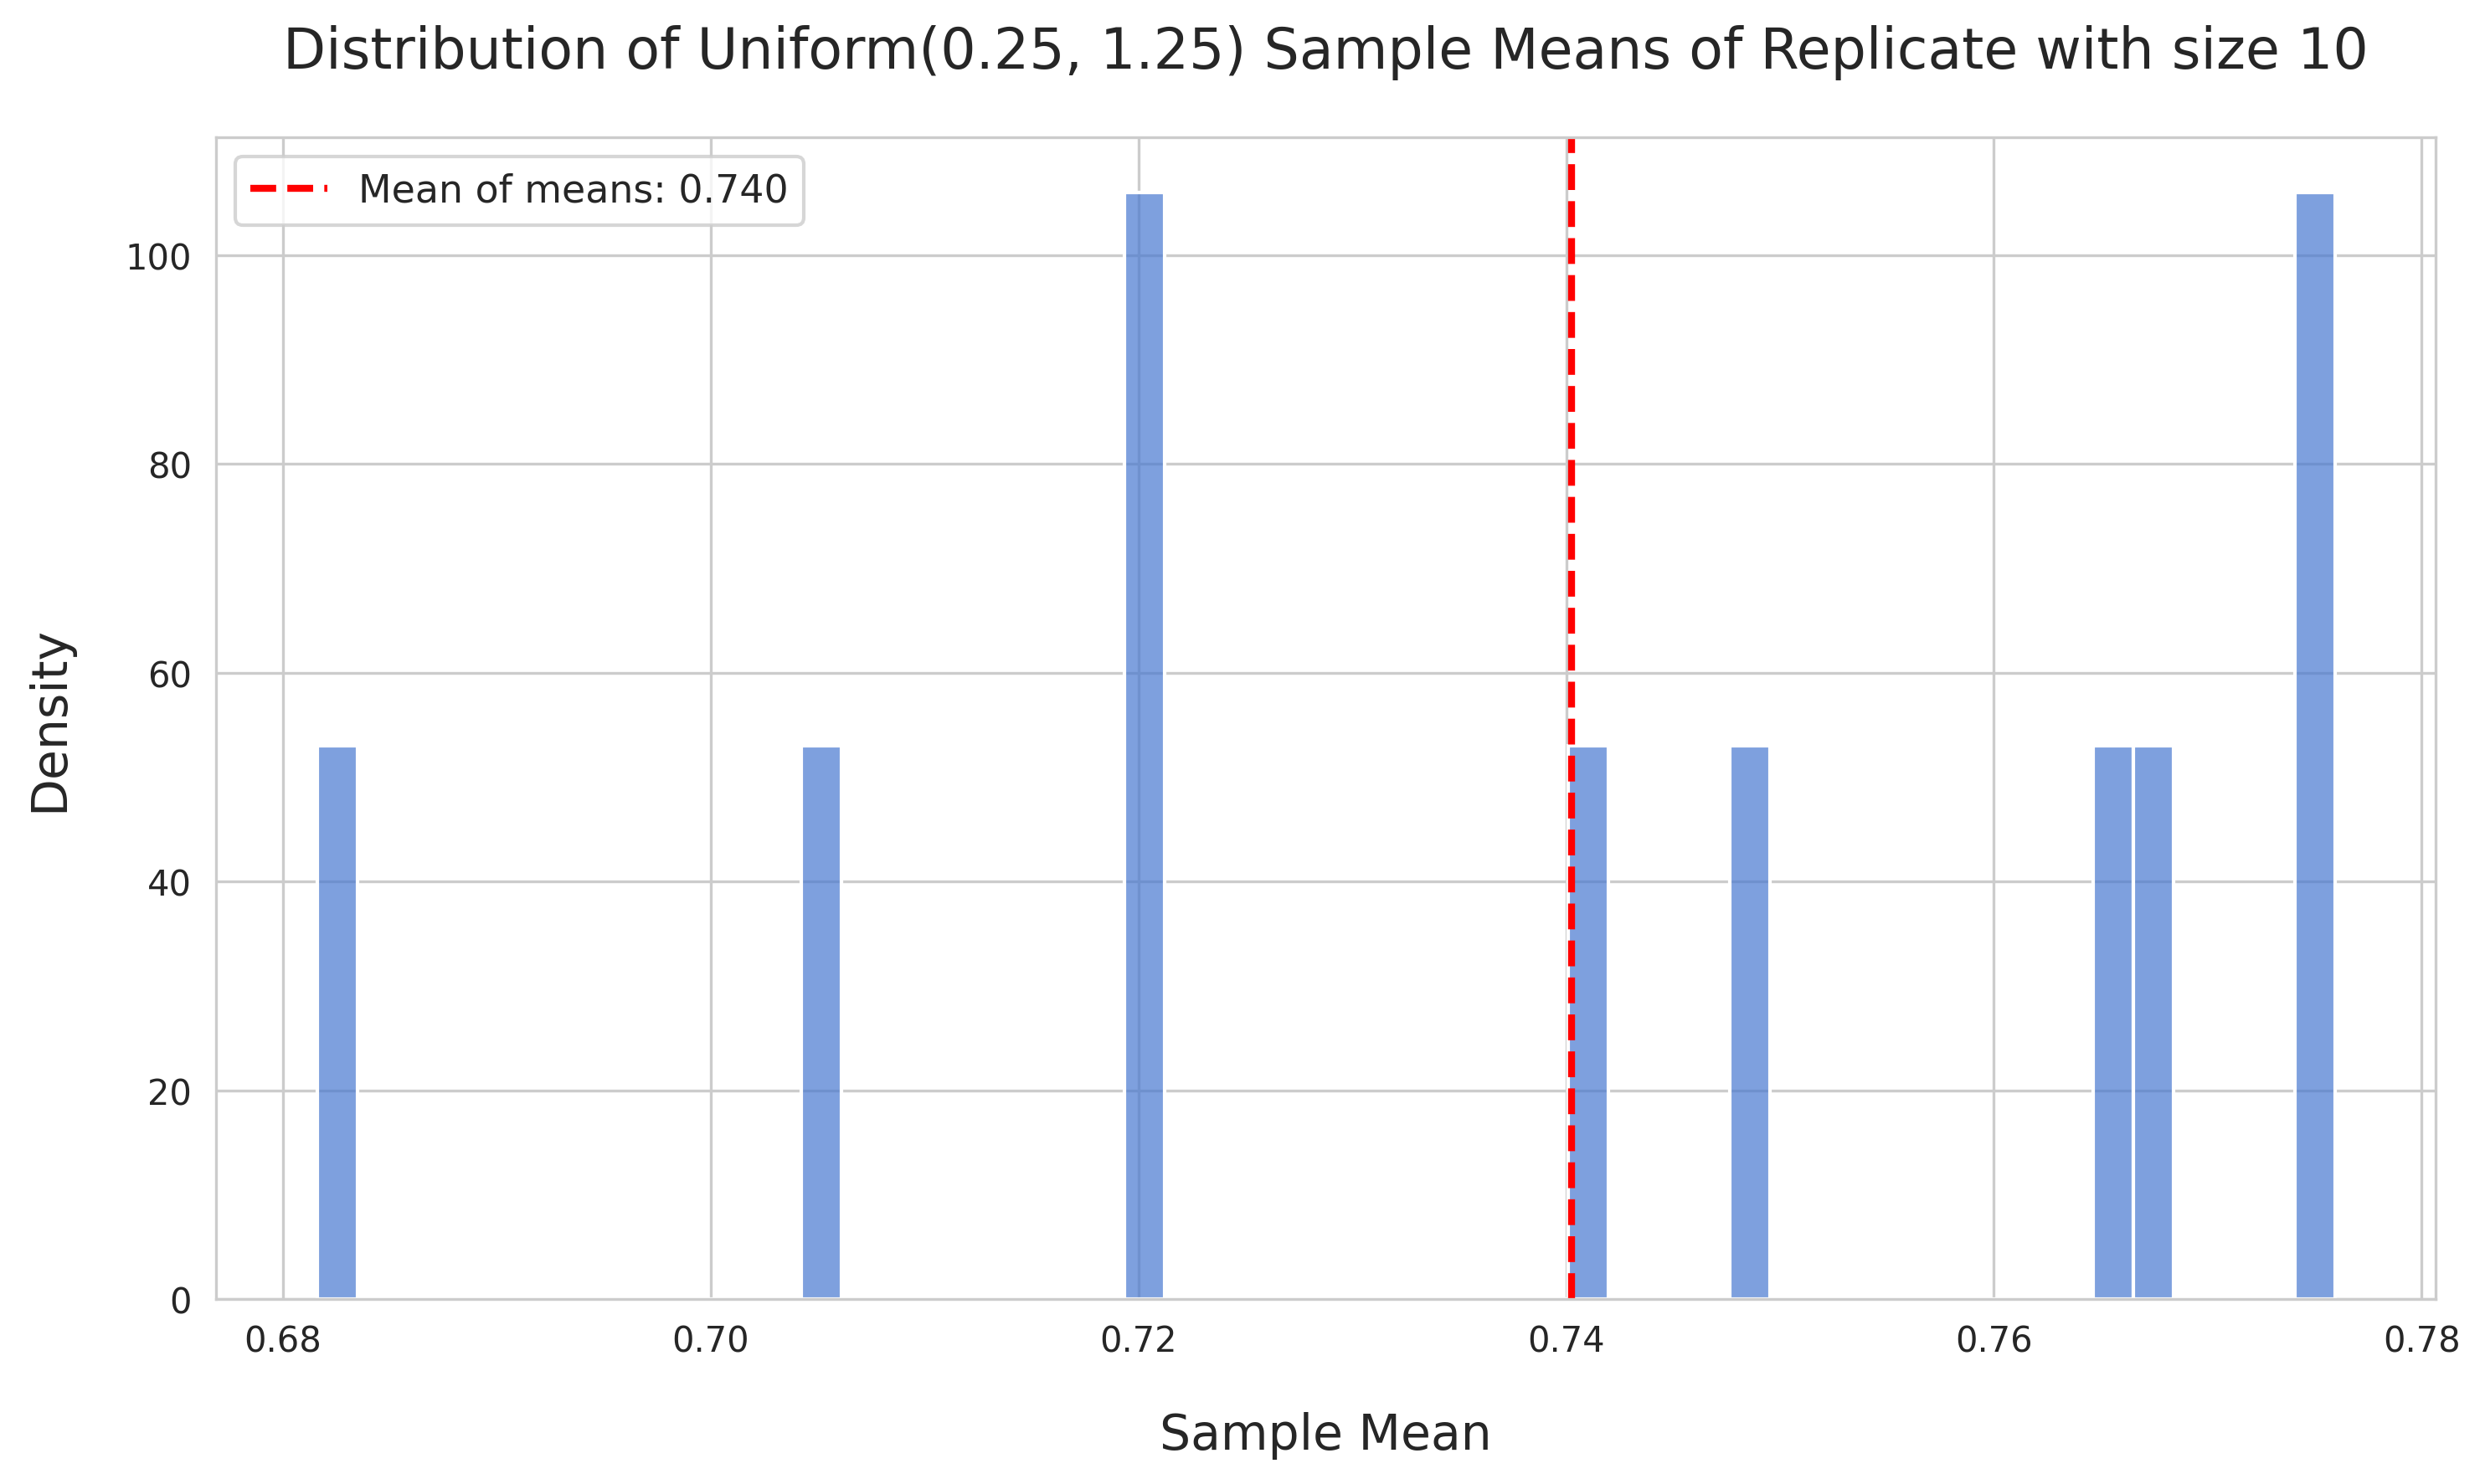
\includegraphics[width=0.95\textwidth]{figures/uniform_sample_means_n10.png}
  
  \textbf{Figure 7:} Distribution of sample means from Uniform(0.25, 1.25) with replicate size 10.
\end{center}

\begin{center}
  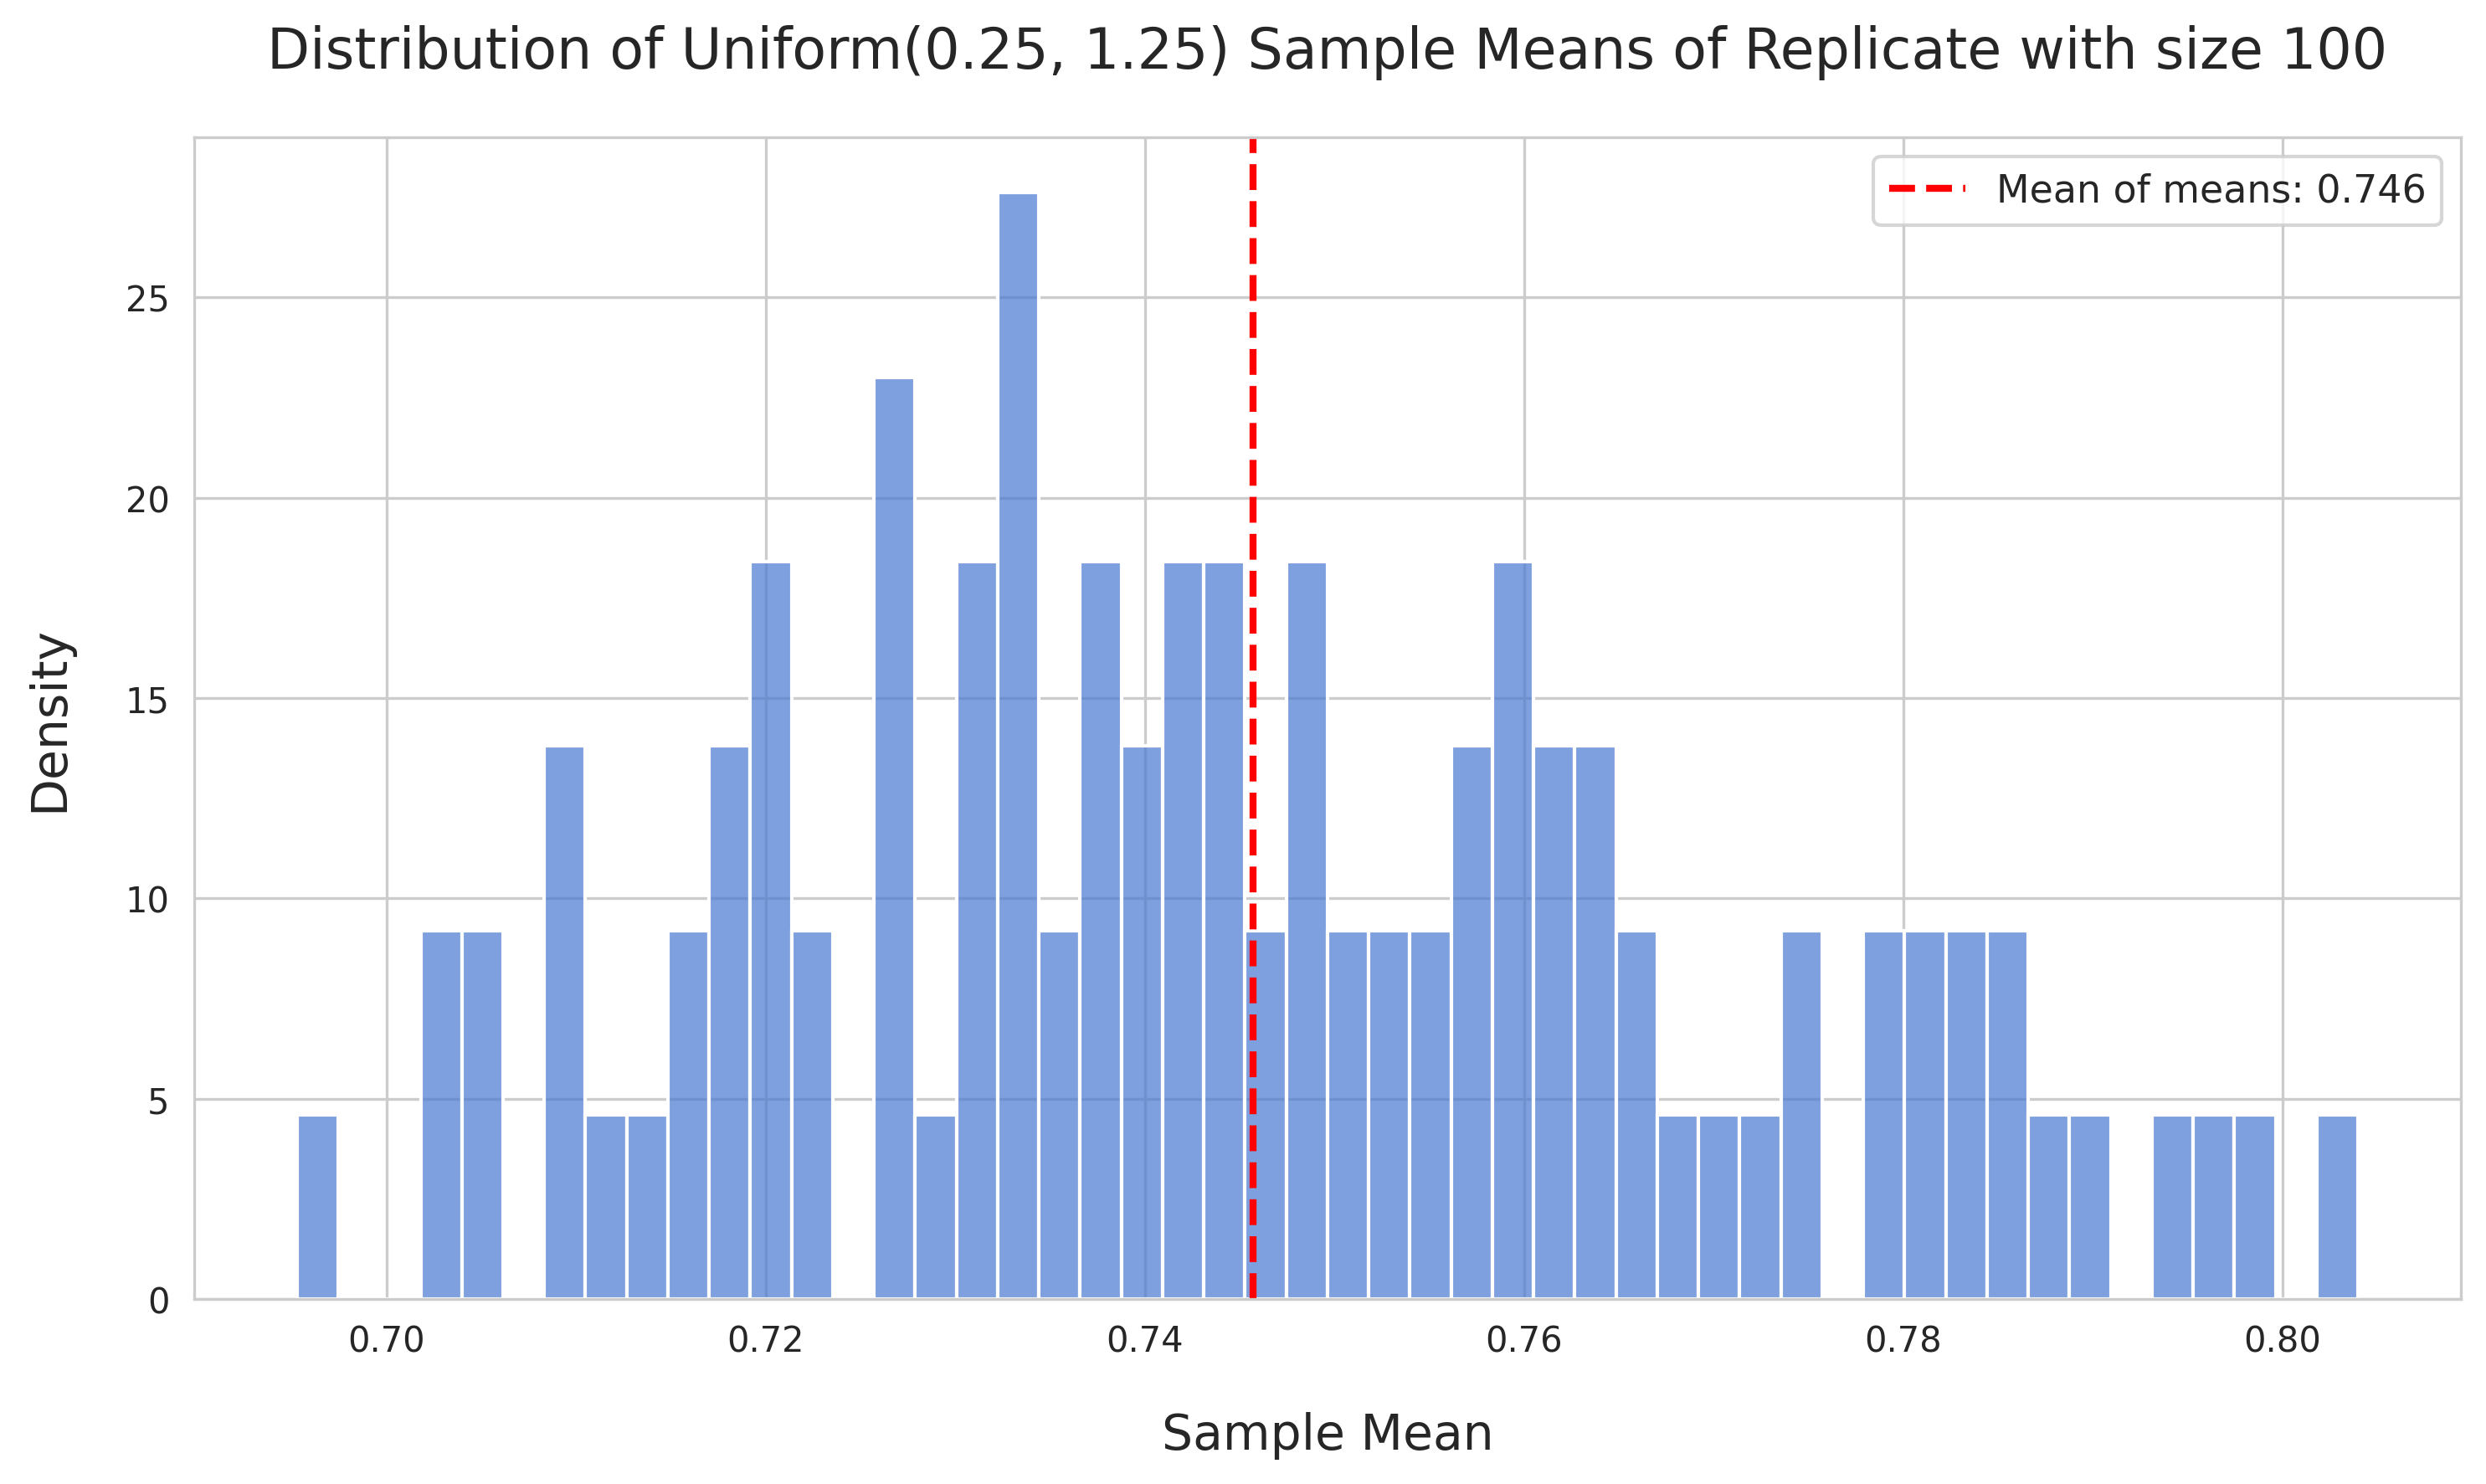
\includegraphics[width=0.95\textwidth]{figures/uniform_sample_means_n100.png}
  
  \textbf{Figure 8:} Distribution of sample means from Uniform(0.25, 1.25) with replicate size 100.
\end{center}

\begin{center}
  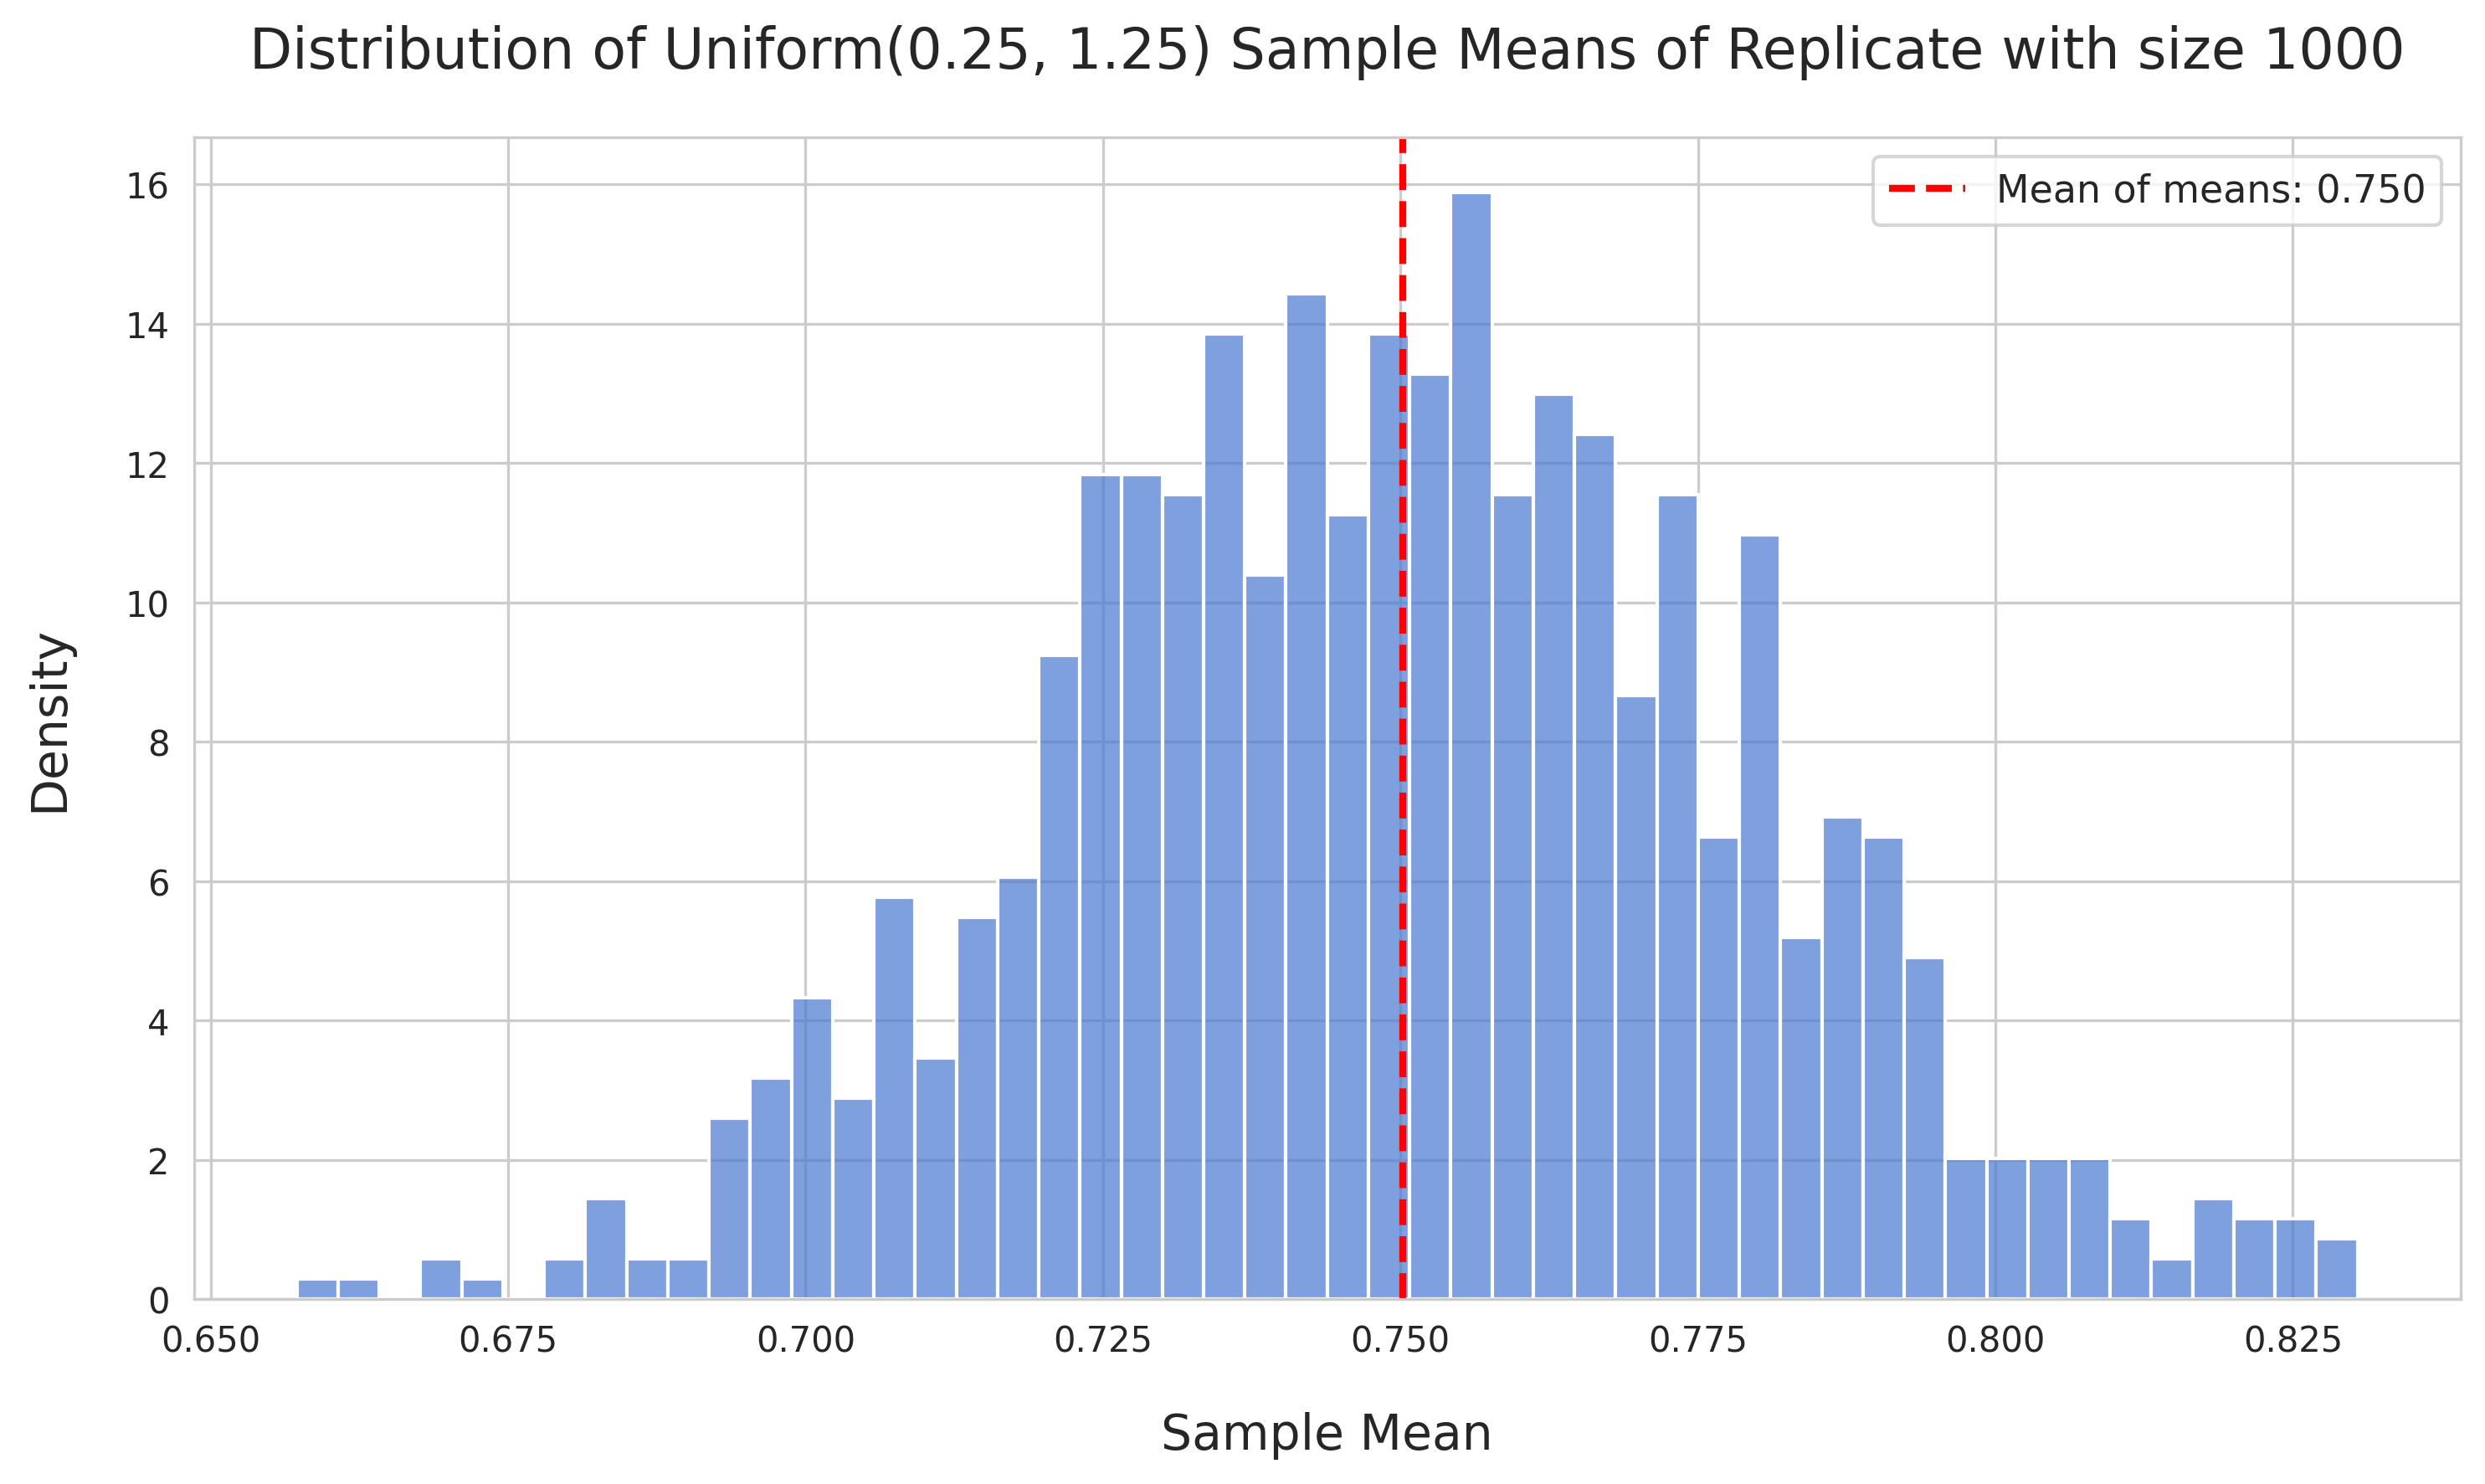
\includegraphics[width=0.95\textwidth]{figures/uniform_sample_means_n1000.png}
  
  \textbf{Figure 9:} Distribution of sample means from Uniform(0.25, 1.25) with replicate size 1000.
\end{center}

Regarding the Uniform sample mean plots, we see the first plot begin with a very rough estimate of population mean from just 10 separate datasets, and we do not yet see a clear distribution. The second plot starts to take on form and shows a more accurate estimation of population mean. We can see the general shape of a Gaussian, which is then confirmed in the third plot, centered around 0.75, equal to $\frac{1.25 + 0.25}{2}$.

\begin{center}
  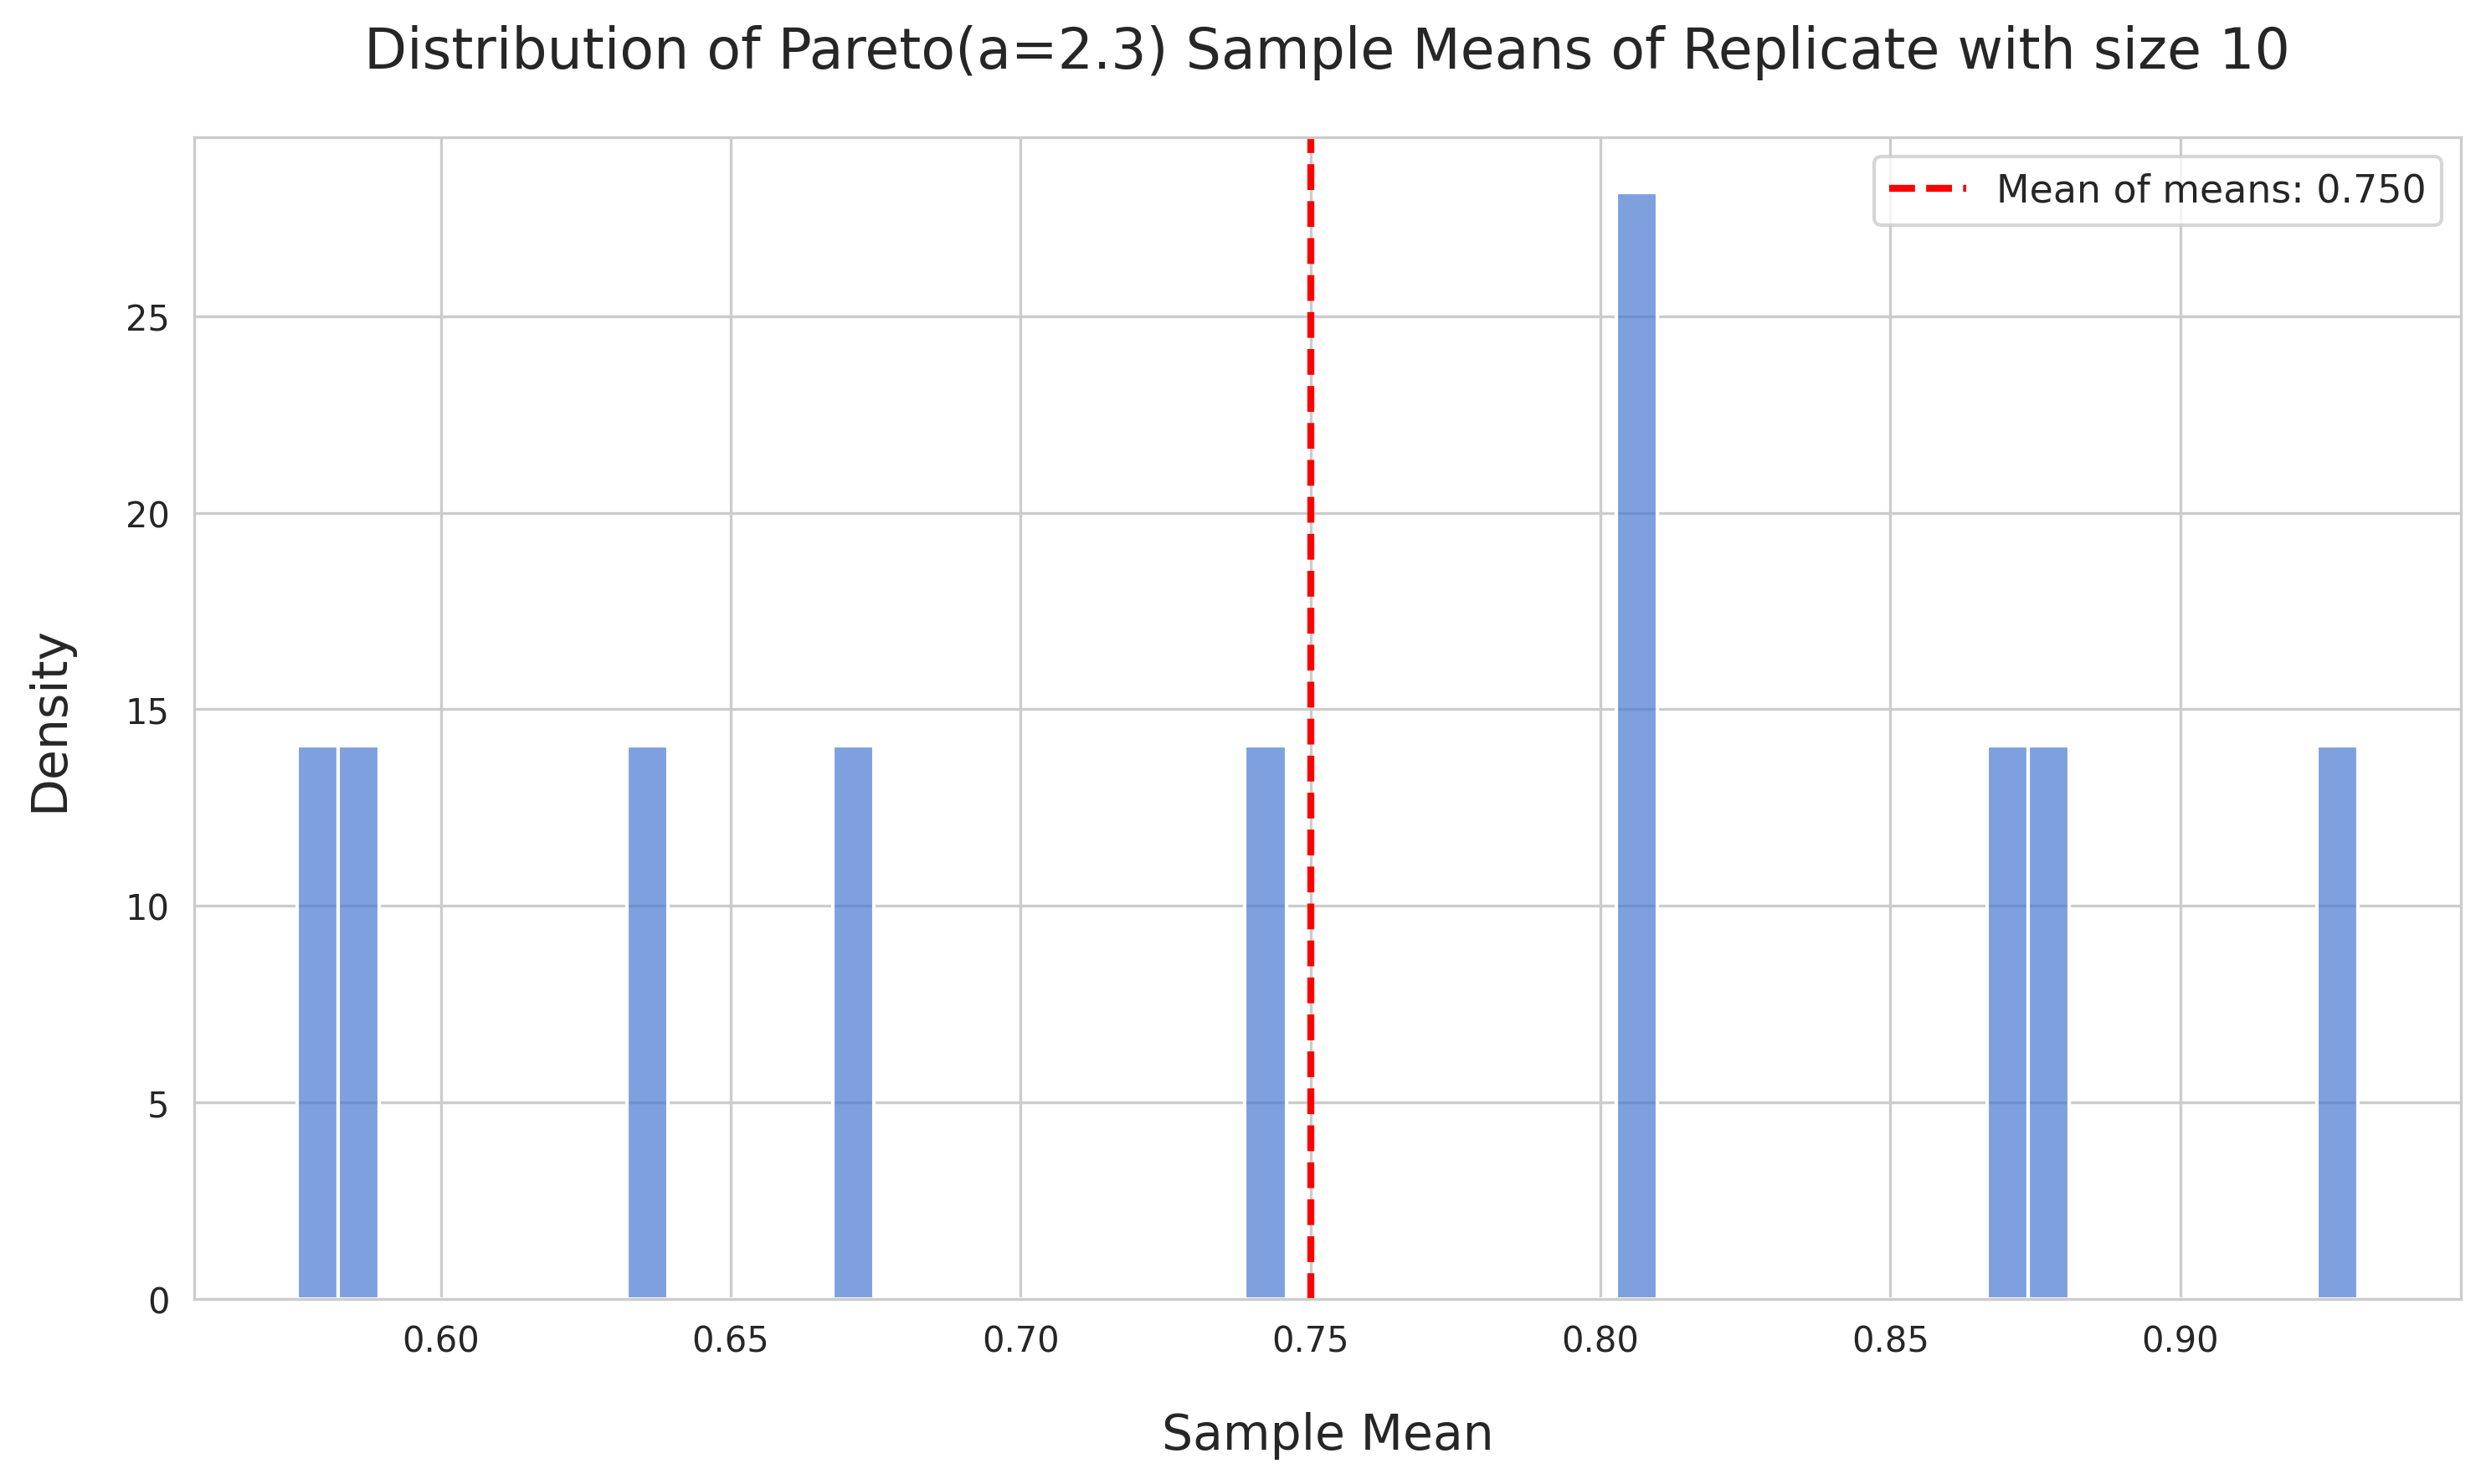
\includegraphics[width=0.95\textwidth]{figures/powerlaw_sample_means_n10.png}
  
  \textbf{Figure 10:} Distribution of sample means from Pareto(a=2.3) with replicate size 10.
\end{center}

\begin{center}
  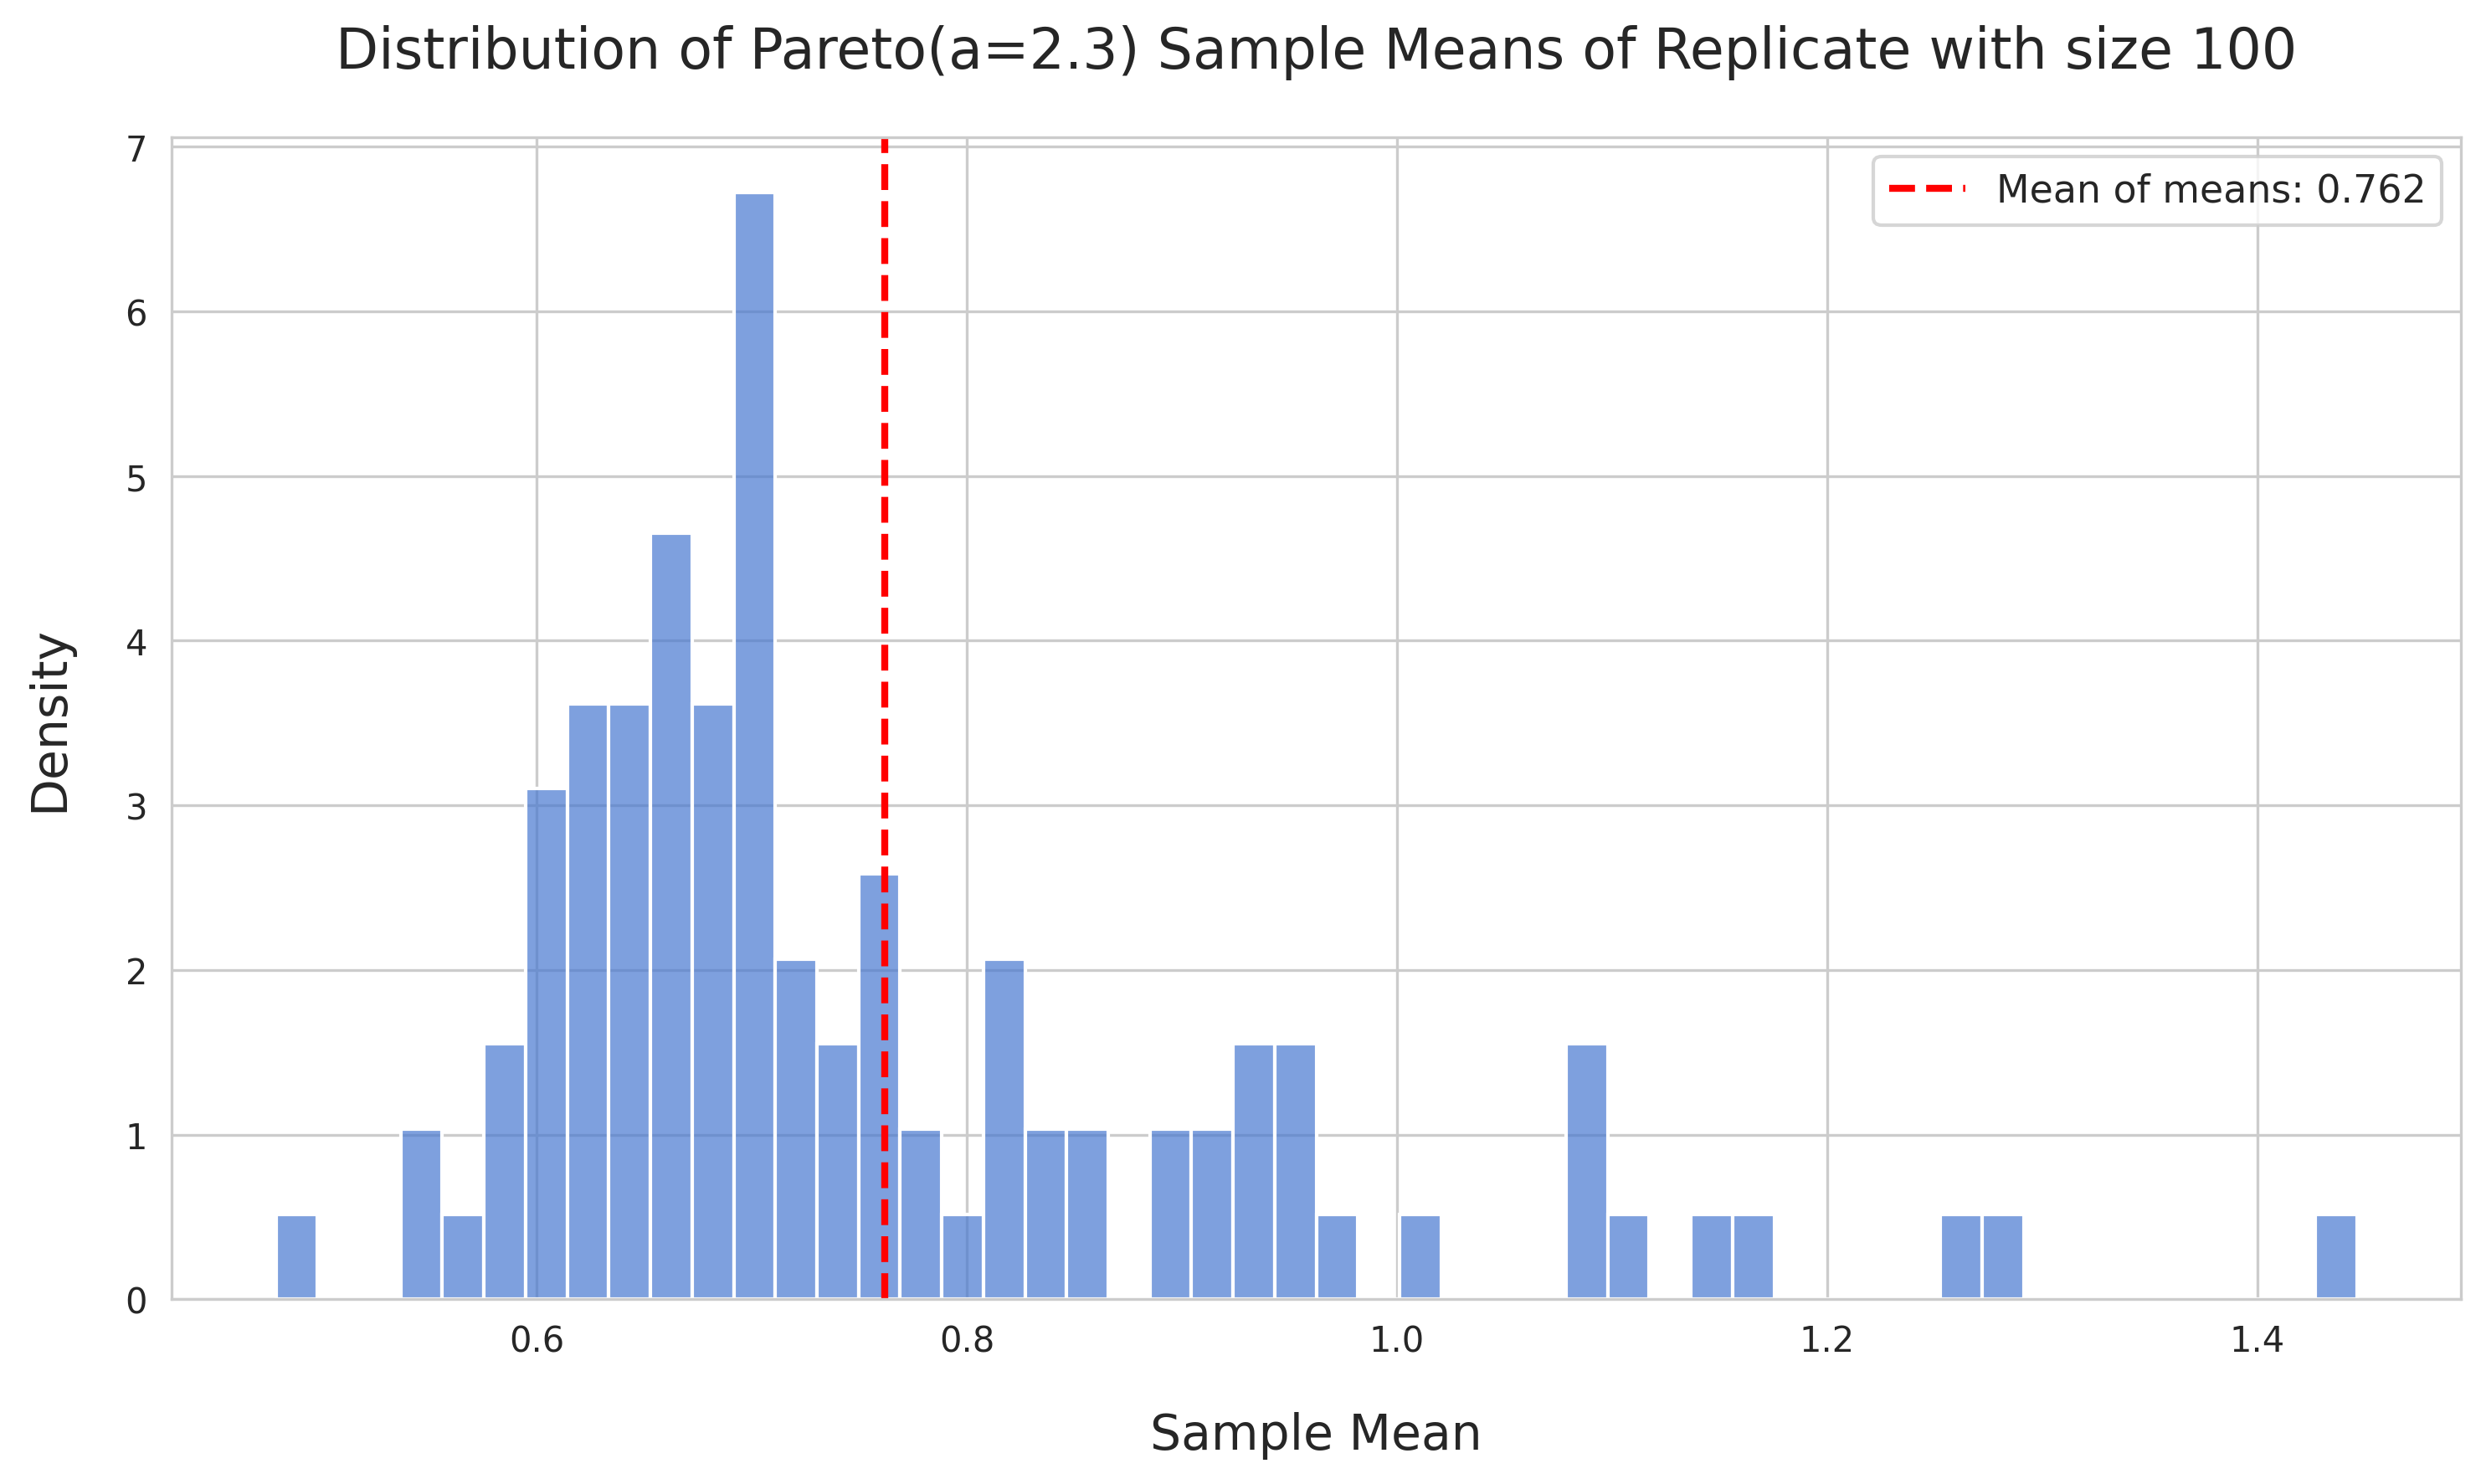
\includegraphics[width=0.95\textwidth]{figures/powerlaw_sample_means_n100.png}
  
  \textbf{Figure 11:} Distribution of sample means from Pareto(a=2.3) with replicate size 100.
\end{center}

\begin{center}
  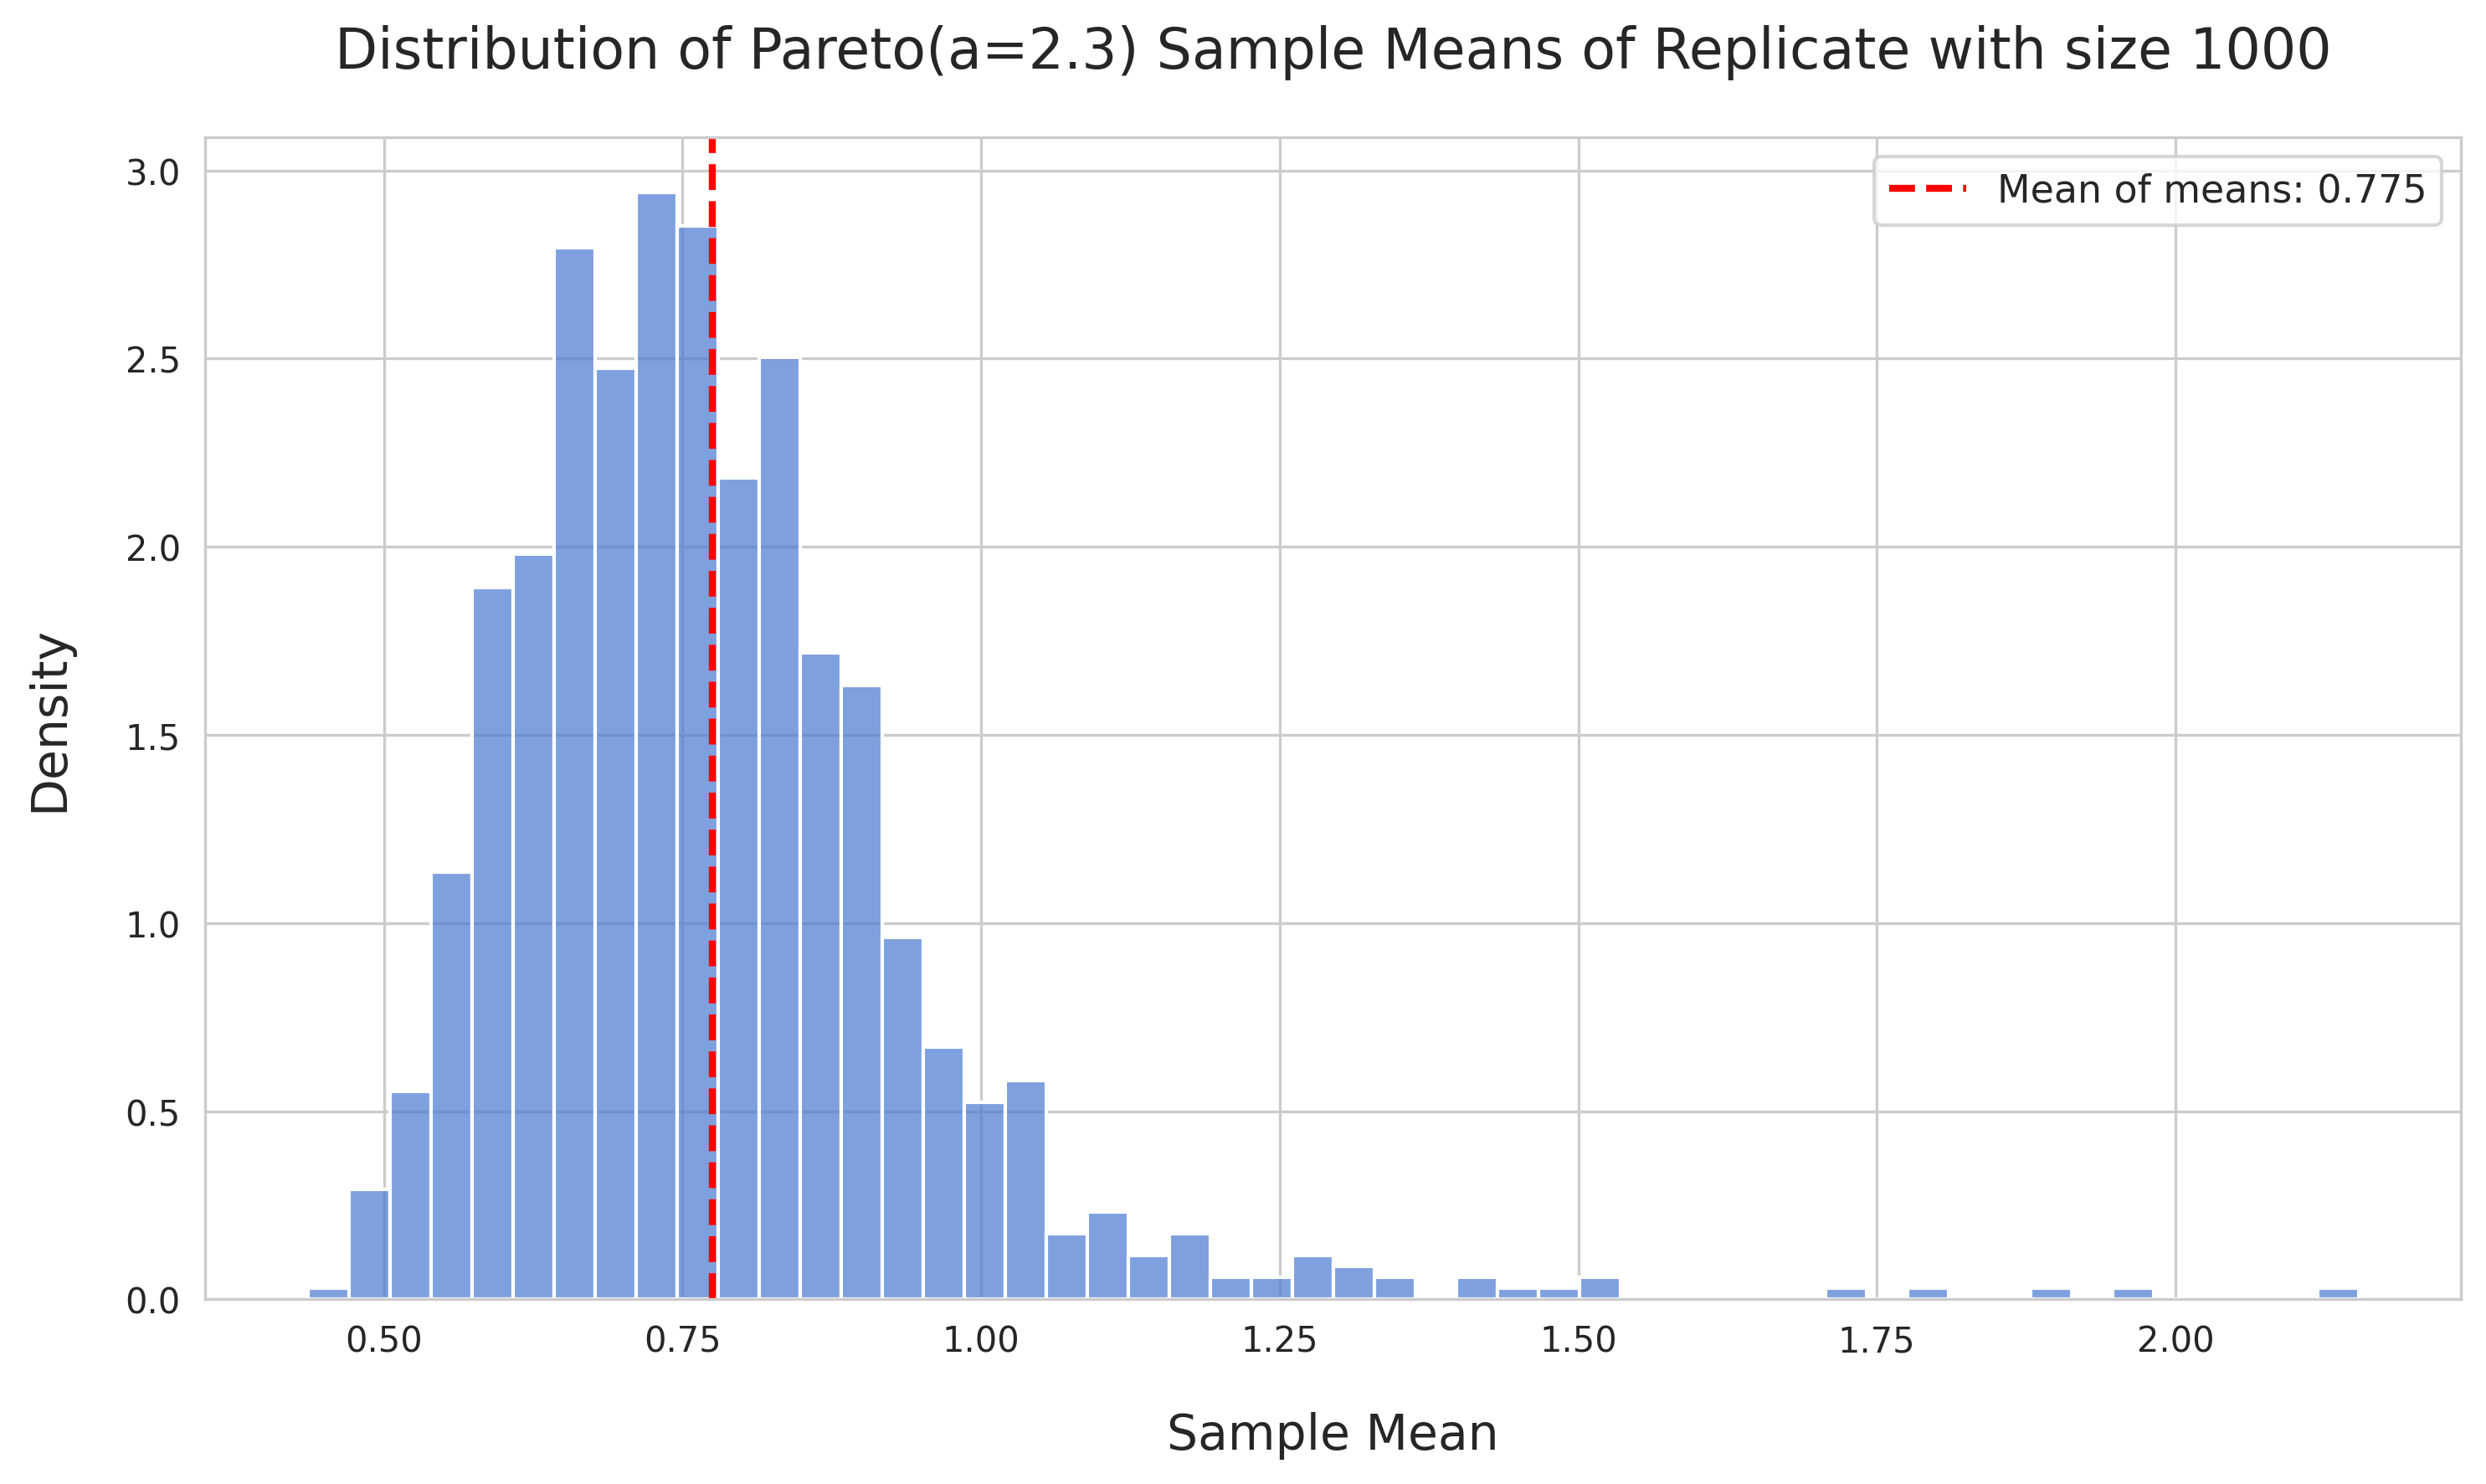
\includegraphics[width=0.95\textwidth]{figures/powerlaw_sample_means_n1000.png}
  
  \textbf{Figure 12:} Distribution of sample means from Pareto(a=2.3) with replicate size 1000.
\end{center}

The Pareto sample mean plots show a similar convergence, though for the smaller two replicate sizes we have a number of datasets that tend to possess more of the predictable extreme values of the Power-Law distribution than others, causing a right skew in the distribution mass that mellows out only with increased number of sample means. The final plot shows a convergence toward a fairly smooth Gaussian, centered around 0.775, even if much slower due to its proclivity toward occasional extremes.\\

So regardless of the distribution type, we have at least a visual confirmation that CLT is applying appropriately to both, though the convergence of the sample means to a Gaussian as it relates to the number of samples may be influenced by the properties of the specific distributions in question.

\newpage
